%==============================================================================
% TEMPLATE FOR THESIS WAGENINGEN UNIVERSITY
% CREATED BY AREND LIGTENBERG JUNE 2006;
% EDITED BY KIM CALDERS 2014;
% EDITED BY BEN DEVRIES 2015;
% EDITED BY LOIC DUTRIEUX 2016;
% EDITED BY BENJAMIN BREDE 2019;
% EDITED BY DAINIUS MASILIUNAS 2023;
%==============================================================================

\documentclass [a4paper,12pt,twoside]{book}
% PDFLaTeX options only; disable for XeLaTeX
\usepackage[utf8]{inputenc}
\usepackage[T1]{fontenc}
% End PDFLaTeX options
\usepackage[dutch,english]{babel}
\usepackage{graphicx}
\usepackage{amsmath}
\usepackage{fancyhdr}
\usepackage[small,bf]{caption}
\usepackage{multirow}
\usepackage[top=3.35cm, bottom=3.35cm, left=2.5cm, right=2.5cm]{geometry}
\usepackage[parfill]{parskip}
%\usepackage{pdfpages}
\usepackage{color}
\usepackage{appendix}

% extra packages added by Ben
\usepackage{rotating} % for rotating figures
\usepackage{changepage} % for indenting entire paragraphs
\usepackage{float} % help with table positioning
\floatstyle{plaintop} % caption on top
\restylefloat{table} % see above. Use: \begin{table}[H]
\usepackage{csquotes} % for block quotes, use {displayquote} environment
\usepackage{todonotes}
\usepackage{fp}
\usepackage{tabularx}
\usepackage{pdflscape}

% extra packages added by Ben B
\usepackage{booktabs} 
\usepackage{microtype} % fancy typesetting
\usepackage[plain]{fancyref} % fancy cross-references
\usepackage{enumitem} % flexible numeration/list environments
\usepackage{pageslts} % to get total number of pages for frontmatter
\usepackage{etoolbox} % to fix acronym macro

% Extra packages added by Dainius
\usepackage{adjustbox} % For resizing tables
\usepackage{wrapfig} % For picture of the author in biography
\newcommand{\sep}{, } % Definition from elsarticle for ease of portability
\newcommand{\minisection}[1]{\paragraph{#1.}} % Section that does not appear in TOC and without a new line after it
\newcommand{\cran}[1]{\texttt{#1}} % Elsevier papers ask to indicate repositories, but here we just do a texttt
% Start of subappendices environment
\AtBeginEnvironment{subappendices}{%
%    \section*{Appendices}
    \counterwithin{figure}{section}
    \counterwithin{table}{section}
}
% End of subappendices environment
\AtEndEnvironment{subappendices}{%
    \counterwithout{figure}{section}
    \counterwithout{table}{section}
    \counterwithin{figure}{chapter}
    \counterwithin{table}{chapter}
}
%\usepackage[11-18,67-78,85-88]{pagesel}

%%%% Add an edge index
\usetikzlibrary{calc}
% auxiliary counter
\newcounter{chapshift}
\addtocounter{chapshift}{-1}

% the list of colors to be used (add more if needed)
\newcommand\BoxColor{%
  \ifcase\thechapshift gray\or gray\or gray\or gray\or gray\else gray\fi}

\newif\ifedgeindex
\edgeindextrue
% the main command; the mandatory argument sets the color of the vertical box
\newcommand\EdgeIndexChapter{%
  \AddToHook{shipout/background}{%
    \ifedgeindex
        \ifodd\value{page}
          {%
          \put (\paperwidth-1.3cm, \numexpr\thechapshift*-3-3\relax cm) {
            \begin{tikzpicture}
              \node[
                fill=\BoxColor,
                inner sep=0pt,
                rectangle,
                text width=0.8cm,
                minimum height=3cm,
                minimum width=1.6cm,
                align=left,
                anchor=north east
              ] 
              {\center\bfseries\LARGE\color{white}\thechapter};
            \end{tikzpicture}%
          }%
        }  
        \else
          \put (-0.6cm, \numexpr\thechapshift*-3-3\relax cm) {
          {%
            \begin{tikzpicture}
            \node[
              fill=\BoxColor,
              inner sep=0pt,
              rectangle,
              text width=0.8cm,
              minimum height=3cm,
              minimum width=1.6cm,
              align=right,
              anchor=north west
            ] 
            {\center\bfseries\LARGE\color{white}\thechapter};
            \end{tikzpicture}%
          }%
        }  
        \fi
    \fi
  }%
  \stepcounter{chapshift}%
}

\newcommand\RemoveEdgeIndex{\edgeindexfalse}

% Add crop marks due to the edge index; remove this for a clean PDF for sending to others
% Calculation is: with bleed it is 18x25, the scale factor from A4 to 17x24 is 0.8088023, therefore 18/0.808 x 25/0.808
\usepackage[width=22.26truecm, height=30.91truecm, center]{crop}
% set "cross, color=red" to see the cut marks
% mount2 would add bleed only to the outside, but PM does not need that.

%\WarningsOff[xeCJK]
%\WarningsOff[fontspec]
%\usepackage{xeCJK} % For CJK character support; this requires XeLaTeX!
\usepackage{CJKutf8}

% make \url{} command available in text, break urls at hyphens (important for bibliography)
\PassOptionsToPackage{hyphens}{url}
\usepackage[bookmarksdepth=2,colorlinks=false,hidelinks,pdfusetitle]{hyperref}
\usepackage{url}

% bibliography with biblatex
\usepackage[
	backend=biber,
	natbib, % allow natbib cite commands
	alldates=year,
	style=authoryear,
	sorting=nyt, % sorting order of the bibs: name, year, title
        % ISSUE: it sorts my full author list and then by year. style=alphabetic does not help because it sorts only on first letter of first author.
	sortcites, % sort in cite, when multiple refs are cited
	giveninits, % abbreveate first names
        useprefix=true, % support Dutch "van der" surname prefix
	maxbibnames=100, % max names per biobliography entry
	minbibnames=13,
	maxcitenames=2, % max names per citation
	uniquelist=false, % force inline citations to have no first names or additional co-authors
	uniquename=false, % force inline citations to have no first names or additional co-authors
	hyperref=true,
	doi,
	isbn=false
]{biblatex}

% add bib databases and give them unique labels to later refer to them
% paths can be absolute
% published papers of the PhD should be in both refs (or refsAdditional) and mypubs
\addbibresource[label=refs]{refs.bib}
\addbibresource[label=refsAdditional]{moreRefs.bib}
% use author+an field in ownPublications.bib to specify which author should be highlighted
\addbibresource[label=mypubs]{ownPublications.bib}

% biblatex + Mendeley/Zotero: ignore some fields produced by Mendeley that are not biblatex conform (or not necessary)
\DeclareSourcemap{
	\maps[datatype=bibtex, overwrite]{
		\map{
			\perdatasource{refs}
			\step[fieldset=ISBN, null]
			\step[fieldset=month, null]
			\step[fieldset=abstract, null]
			\step[fieldset=file, null]
			\step[fieldset=keywords, null]
			\step[fieldset={mendeley-tags}, null]
			\step[fieldset=number, null]
			\step[fieldset=urldate, null]
			\step[fieldset=language, null]
		}
		\map{
			\perdatasource{refsAdditional}
			\step[fieldset=ISBN, null]
			\step[fieldset=month, null]
			\step[fieldset=abstract, null]
			\step[fieldset=file, null]
			\step[fieldset=keywords, null]
			\step[fieldset={mendeley-tags}, null]
			\step[fieldset=number, null]
			\step[fieldset=urldate, null]
			\step[fieldset=language, null]
		}
		\map{
			\pernottype{manual}
			\step[fieldset=url, null] % remove urls from all but manual > DOI has same information content
		}
	}
}

% add space between bibliography items
\setlength\bibitemsep{0.25\baselineskip}

% use all authors for fullcite
\preto\fullcite{\AtNextCite{\defcounter{maxnames}{99}}} 
%https://tex.stackexchange.com/questions/126226/how-do-i-instruct-fullcite-to-use-maxbibnames-rather-than-maxcitenames

% for biblatex + own publication list: make author name bold if annotated (bibtex field author+an in mypubs.bib)
\renewcommand*{\mkbibnamegiven}[1]{%
	\ifitemannotation{highlight}
	{\textbf{#1}}
	{#1}
}
\renewcommand*{\mkbibnamefamily}[1]{%
	\ifitemannotation{highlight}
	{\textbf{#1}}
	{#1}
}

% in bibliography: remove "in:" before journal names for articles
\renewbibmacro{in:}{%
	\ifentrytype{article}{}{\printtext{\bibstring{in}\intitlepunct}}
}

% in bibliography: removes pagination (p./pp.) before page numbers
\DeclareFieldFormat{pages}{#1}


% typeset units correctly
\usepackage{siunitx} 
\sisetup{range-units=single, separate-uncertainty=true, multi-part-units=repeat, detect-weight=true}
\DeclareSIUnit \lai{ \square\metre\per\square\metre }

\usepackage[labelformat=simple]{subcaption}
\renewcommand\thesubfigure{\alph{subfigure}}
\DeclareCaptionLabelFormat{subcaptionlabel}{\normalfont(\textbf{#2}\normalfont)}
%\captionsetup[subfigure]{labelformat=subcaptionlabel}

% full acronyms once, then abbreviations
\usepackage[acronym,toc,shortcuts]{glossaries} 
\makenoidxglossaries
\newacronym{NDVI}{NDVI}{Normalised Difference Vegetation Index}


%\addto\captionsenglish{\renewcommand{\bibname}{References}} % REFERENCES > References

\widowpenalty10000
\clubpenalty10000

% allow up to 80% of page to be float (figure/table) and still print text
\renewcommand{\floatpagefraction}{.8}

\definecolor{Red}{rgb}{0.5,0,0}
\definecolor{Blue}{rgb}{0,0,0.5}


%=======================================================================
% GENERAL SETTINGS
%=======================================================================
%\oddsidemargin 40pt
%\evensidemargin 40pt
\setlength{\captionmargin}{5pt}
%\setlength{\textfloatsep}{10pt plus 1.0pt minus 2.0pt}
%\usepackage{pifont}
%\usepackage{times}
%\usepackage{txfonts}
%\usepackage[sc]{mathpazo}
%\usepackage{setspace}

\linespread{1.1} %1 is single spacing, 1.3 is oneandhalf spacing


%\citationstyle{dcu}
\sloppy
\setcounter{tocdepth}{0}

%% for internal use
\newcommand{\fixme}[1]{\emph{\marginpar{FIXME} (#1)}}
\newcommand{\readme}[1]{\emph{\marginpar{README} (#1)}}
\newcommand{\verifyme}[1]{\emph{\marginpar{VERIFYME} (#1)}}


%=======================================================================
% DEFINITION OF THE FANCY HEADERS
%=======================================================================
\pagestyle{fancy}
\renewcommand{\chaptermark}[1]{\markboth{#1}{}}
\renewcommand{\sectionmark}[1]{\markright{\thesection\ #1}}
\fancyhf{}
\fancyhead[LE,RO]{\bfseries\thepage}
\fancyhead[LO]{\bfseries\nouppercase{\rightmark}}
\fancyhead[RE]{\bfseries\nouppercase{\leftmark}}
%\fancyfoot[LE,CE,RE]{\scriptsize{Draft: June 2006}}
%\fancyfoot[LO,CO,RO]{\scriptsize{Draft: June 2006}}
\headheight 15pt

\fancypagestyle{plain}{%
	\fancyhead{} % get rid of headers
	\renewcommand{\headrulewidth}{0pt} % and the line
}
\renewcommand{\headrulewidth}{0.4pt}
%\renewcommand{\footrulewidth}{0.4pt}

%==============================
% Metadata of the thesis
%==============================

% Variables defining the metadata of the thesis
% Fill here once and it will be used throughout the document

\newcommand{\thetitle}{Title of your Thesis}
\newcommand{\theauthor}{John Doe}
\newcommand{\defencedate}{01 January 2025}
\year=2025
\newcommand{\defencetime}{1:30 p.m.}
\newcommand{\firstpromotor}{Prof. Dr J. Smith}


\title{\thetitle}
\author{\theauthor}

%=======================================================================
% NEW ENVIRONMENT FOR THE START OF CHAPTER (SMALL ABSTRACT)
%=======================================================================
%\newenvironment{chapintro}
%{
%    \begin{center}
%    \begin{minipage}[t]{0.9\textwidth}
%    \hrule
%    \medskip
%    \small
%}
%{
%    \medskip
%    \hrule
%    \end{minipage}
%    \end{center}
%    \bigskip
%}


%=======================================================================
% ADD WORD CHAPTER FOR TOC
%=======================================================================


\makeatletter
\let\orig@chapter\@chapter
\def\@chapter[#1]#2{\ifnum \c@secnumdepth >\m@ne
                       \if@mainmatter
                         \refstepcounter{chapter}%
                         \typeout{\@chapapp\space\thechapter.}%
                         \addcontentsline{toc}{chapter}%
                                   {Chapter~\protect\numberline{\thechapter}#1}%
                       \else
                         \addcontentsline{toc}{chapter}{#1}%
                       \fi
                    \else
                      \addcontentsline{toc}{chapter}{#1}%
                    \fi
                    \chaptermark{#1}%
                    \addtocontents{lof}{\protect\addvspace{10\p@}}%
                    \addtocontents{lot}{\protect\addvspace{10\p@}}%
                    \if@twocolumn
                      \@topnewpage[\@makechapterhead{#2}]%
                    \else
                      \@makechapterhead{#2}%
                      \@afterheading
                    \fi}
% allow hyphenation of acronyms                
\patchcmd\AC@acs{\mbox}{\@firstofone}{}{} 

\makeatother

% Allow numbering for subsubsections
\setcounter{secnumdepth}{3}

%=======================================================================
% A BIT MORE COMPACT ITEM LIST
%=======================================================================
%\newenvironment{itemize*}%
%  {\begin{itemize}%
%    \setlength{\parskip}{0pt}%
%    \setlength{\itemsep}{0pt}%
%    \setlength{\parsep}{0pt}}%
%  {\end{itemize}}
%
%%more compact enumeration list
%  \newenvironment{enumerate*}%
%  {\begin{enumerate}%
%    \setlength{\itemsep}{0pt}%
%    \setlength{\parskip}{0pt}}%
%  {\end{enumerate}}

%=======================================================================
% A BIT MORE COMPACT DESCRIPTION LIST
%=======================================================================
%\renewcommand{\descriptionlabel}[1]{\hspace{\labelsep}\textrm{#1}}
%
%\newenvironment{description*}%
%  {\begin{description}%
%    \setlength{\itemsep}{0pt}%
%    \setlength{\parskip}{0pt}}%
%  {\end{description}}


%=======================================================================
% CLEAR HEADER STYLE ON LAST EMPTY ODD PAGES
%=======================================================================
\makeatletter
\def\cleardoublepage{\clearpage\if@twoside \ifodd\c@page\else%
\hbox{}%
\thispagestyle{empty}%
\newpage%
\if@twocolumn\hbox{}\newpage\fi\fi\fi}
\makeatother


%=======================================================================
% SOME EXTRA COMMANDS FOR VISUAL LAYOUT
%=======================================================================
\newcommand{\longpage}{\enlargethispage{\baselineskip}}
\newcommand{\shortpage}{\enlargethispage{-\baselineskip}}
\newcommand{\setreference}{\vspace*{\fill}}


%==============================
% REFORMAT SECTION HEADINGS
%==============================

%% using titlesec
\usepackage{titlesec}
%% FIX FOR BUG in titlesec 2.10.1
%\usepackage{etoolbox}

%\makeatletter
%\patchcmd{\ttlh@hang}{\parindent\z@}{\parindent\z@\leavevmode}{}{}
%\patchcmd{\ttlh@hang}{\noindent}{}{}{}
%\makeatother
%% END OF BUGFIX

\titleformat{\subsection}
  {\normalfont\normalsize\bfseries}
  {\thesubsection}{1em}{}
\titleformat{\subsubsection}
  {\normalfont\normalsize\itshape}
  {\thesubsubsection}{1em}{}



%==============================
% Force start of newpage on left page
%==============================
\newcommand*\cleartoleftpage{%
  \clearpage
  \ifodd\value{page}\hbox{}\newpage\fi
}

%=======================================================================
% INCLUSION OF THE CONTENT
%=======================================================================

\raggedbottom % preferentially leaves whitespace at bottom of page instead of distributing throughout vertical space

\begin{document}

\frontmatter
%\pagenumbering{alph}
\pagenumbering{roman}
\addtocontents{toc}{~\hfill\rlap{\textbf{Page}}\par}
\thispagestyle{empty}
%%%%%%%%%%%%%%%%%%%%%%%%%%%%%%%%%%%%%%%%%%%%%%%%%%%%%%%%%%%%%%%%%%
\begin{center}
\Huge{\textbf{\thetitle}} \\
\vspace*{1cm}
\vspace*{1cm}
\vspace*{\fill}
\large{\theauthor}\\
\end{center}

%%%%%%%%%%%%%%%%%%%%%%%%%%%%%%%%%%%%%%%%%%%%%%%%%%%%%%%%%%%%%%%%
\newpage
\thispagestyle{empty}
\vspace*{\fill}

    \textbf{Thesis committee} \\
    \\  
    \textbf{Promotor:} \\
    \firstpromotor{} \\
    Professor of Geo-information Science and Remote Sensing \\
    Wageningen University \& Research \\
    \\  
    \textbf{Co-promotors:} \\
    Prof. Dr F. Swartjes \\
    Professor of Phytopathology, \\
    Wageningen University \& Research \\
    \\
    Dr P.A. Willis \\  
    Associate professor, Animal Nutrition Group \\
    Wageningen University \& Research \\
    \\

    \textbf{Other members:}                                                                   \\
    Prof. Dr W.J. Stekels, Wageningen University \& Research \\  
    Dr P. de Groot, University of Amsterdam \\
    Dr A. de Bruin, Keygene N.V., Wageningen \\
    Dr P. van Oost, University of Aberdeen, UK \\
    \\  

    This research was conducted under the auspices of the
    C.T. de Wit Graduate School of Production Ecology \& Resource Conservation (PE\&RC)                         \\

%%%%%%%%%%%%%%%%%%%%%%%%%%%%%%%%%%%%%%%%%%%%%%%%%%%%%%%%%%%%%%%%
\newpage
\thispagestyle{empty}
\begin{center}
\Huge{\textbf{\thetitle}} \\
\vspace*{1cm}
\Large{\theauthor}\\
\normalsize
\vspace*{\fill}
\textbf{Thesis} \\
submitted in fulfilment of the requirements for the degree of doctor at \\
Wageningen University\\
by the authority of the Rector Magnificus\\
Prof. Dr C. Kroeze,\\
in the presence of the\\
Thesis Committee appointed by the Academic Board\\
to be defended in public\\
on \defencedate{}\\
at \defencetime{} in the Omnia Auditorium.\\
\end{center}

%%%%%%%%%%%%%%%%%%%%%%%%%%%%%%%%%%%%%%%%%%%%%%%%%%%%%%%%%%%%%%%%%%%
\newpage
\thispagestyle{empty}
\vspace*{\fill}
\begin{flushleft}
\begin{tabular}{l}
    \theauthor                                               \\
    \thetitle                                     \\
    \lastpageref{LastPages} pages.                           \\  
                                                             \\  
    PhD thesis, Wageningen University, Wageningen, the Netherlands (\the\year{}) \\
    With references, with summary in English                 \\  
                                                             \\  
    DOI: \url{https://doi.org/xx.xxxxx/xxxxxx}
\end{tabular}
\end{flushleft}
%\newpage
%\thispagestyle{empty}
%\begin{flushright}
%\vspace*{\fill}
%\textit{Aan mijn ouders}
%\end{flushright}


\cleardoublepage
\phantomsection
\begin{refsection}[mypubs]
\chapter{Summary}
\label{cha:Summary}

\dots

\textbf{Chapter 1} \dots

\textbf{Chapter 2} \dots

\textbf{Chapter 3} \dots

\textbf{Chapter 4} \dots

\textbf{Chapter 5} \dots

\textbf{Chapter 6} \dots

The PhD thesis \dots

%\pagenumbering{arabic} \setcounter{page}{1}
\end{refsection}

% start refsection: use these specific bib-resources
\begin{refsection}[refs,refsAdditional]

        \cleardoublepage
	\phantomsection
	\addcontentsline{toc}{chapter}{Contents}  
	\tableofcontents
	
	%% Main Chapters
	\mainmatter
	\setcounter{page}{1}
        \EdgeIndexChapter
	\chapter[Introduction]{Introduction}
\label{cha:Chapter1}
\vspace*{\fill}


\newpage

\section{Context}

    Lorem ipsum dolor sit amet, consectetur adipisicing elit, sed do eiusmod
    tempor incididunt ut labore et dolore magna aliqua. Ut enim ad minim veniam,
    quis nostrud exercitation ullamco laboris nisi ut aliquip ex ea commodo \ac{NDVI}
    consequat. Duis aute irure dolor in reprehenderit in voluptate velit esse
    cillum dolore eu fugiat nulla pariatur. Excepteur sint occaecat cupidatat non
    proident, sunt in culpa qui officia deserunt mollit anim id est laborum (figure~\ref{fig:conceptualFramework}).

    \begin{figure}[h]
        \missingfigure{Awesome conceptual framework figure}
        \caption{Conceptual framework}
        \label{fig:conceptualFramework}
    \end{figure}



\section{Thesis Overview}

    Lorem ipsum dolor sit amet, consectetur adipisicing elit, sed do eiusmod
    tempor incididunt ut labore et dolore magna aliqua. Ut enim ad minim veniam,
    quis nostrud exercitation ullamco laboris nisi ut aliquip ex ea commodo \ac{NDVI}
    consequat. Duis aute irure dolor in reprehenderit in voluptate velit esse
    cillum dolore eu fugiat nulla pariatur. Excepteur sint occaecat cupidatat non
    proident, sunt in culpa qui officia deserunt mollit anim id est laborum. % Introduction 
        \EdgeIndexChapter
	\chapter[title of your chapter]{title of your chapter}
\label{cha:chapter1}
\vspace*{\fill}
This chapter is based on:
\\
\\
% Full citation of the published (or submitted/in review) article
% This refers to the article key in the refs.bib file.
\fullcite{Doe2016}
\newpage

\section*{Abstract}
Lorem ipsum dolor sit amet, consectetur adipisicing elit, sed do eiusmod
tempor incididunt ut labore et dolore magna aliqua. Ut enim ad minim veniam,
quis nostrud exercitation ullamco laboris nisi ut aliquip ex ea commodo
consequat. Duis aute irure dolor in reprehenderit in voluptate velit esse
cillum dolore eu fugiat nulla pariatur. Excepteur sint occaecat cupidatat non
proident, sunt in culpa qui officia deserunt mollit anim id est laborum.

\newpage

\section{Introduction}

Lorem ipsum dolor sit amet, consectetur adipisicing elit, sed do eiusmod
tempor incididunt ut labore et dolore magna aliqua. Ut enim ad minim veniam,
quis nostrud exercitation ullamco laboris nisi ut aliquip ex ea commodo
consequat. Duis aute irure dolor in reprehenderit in voluptate velit esse
cillum dolore eu fugiat nulla pariatur. Excepteur sint occaecat cupidatat non
proident, sunt in culpa qui officia deserunt mollit anim id est laborum.

Lorem ipsum dolor sit amet, consectetur adipisicing elit, sed do eiusmod
tempor incididunt ut labore et dolore magna aliqua. Ut enim ad minim veniam,
quis nostrud exercitation ullamco laboris nisi ut aliquip ex ea commodo
consequat. Duis aute irure dolor in reprehenderit in voluptate velit esse
cillum dolore eu fugiat nulla pariatur. Excepteur sint occaecat cupidatat non
proident, sunt in culpa qui officia deserunt mollit anim id est laborum.

\section{Material and methods}

Lorem ipsum dolor sit amet, consectetur adipisicing elit, sed do eiusmod
tempor incididunt ut labore et dolore magna aliqua. Ut enim ad minim veniam,
quis nostrud exercitation ullamco laboris nisi ut aliquip ex ea commodo
consequat. Duis aute irure dolor in reprehenderit in voluptate velit esse
cillum dolore eu fugiat nulla pariatur. Excepteur sint occaecat cupidatat non
proident, sunt in culpa qui officia deserunt mollit anim id est laborum.

\section{Results}

Lorem ipsum dolor sit amet, consectetur adipisicing elit, sed do eiusmod
tempor incididunt ut labore et dolore magna aliqua. Ut enim ad minim veniam,
quis nostrud exercitation ullamco laboris nisi ut aliquip ex ea commodo
consequat. Duis aute irure dolor in reprehenderit in voluptate velit esse
cillum dolore eu fugiat nulla pariatur. Excepteur sint occaecat cupidatat non
proident, sunt in culpa qui officia deserunt mollit anim id est laborum.

\section{Discussion}

Lorem ipsum dolor sit amet, consectetur adipisicing elit, sed do eiusmod
tempor incididunt ut labore et dolore magna aliqua. Ut enim ad minim veniam,
quis nostrud exercitation ullamco laboris nisi ut aliquip ex ea commodo
consequat. Duis aute irure dolor in reprehenderit in voluptate velit esse
cillum dolore eu fugiat nulla pariatur. Excepteur sint occaecat cupidatat non
proident, sunt in culpa qui officia deserunt mollit anim id est laborum.

\section{Conclusions} % (fold)

Lorem ipsum dolor sit amet, consectetur adipisicing elit, sed do eiusmod
tempor incididunt ut labore et dolore magna aliqua. Ut enim ad minim veniam,
quis nostrud exercitation ullamco laboris nisi ut aliquip ex ea commodo
consequat. Duis aute irure dolor in reprehenderit in voluptate velit esse
cillum dolore eu fugiat nulla pariatur. Excepteur sint occaecat cupidatat non
proident, sunt in culpa qui officia deserunt mollit anim id est laborum.

        \EdgeIndexChapter
	\chapter[title of your chapter]{title of your chapter}
\label{cha:chapter2}
\vspace*{\fill}
This chapter is based on:
\\
\\
% Full citation of the published (or submitted/in review) article
% This refers to the article key in the refs.bib file.
\fullcite{Doe2016}
\newpage

\section*{Abstract}
Lorem ipsum dolor sit amet, consectetur adipisicing elit, sed do eiusmod
tempor incididunt ut labore et dolore magna aliqua. Ut enim ad minim veniam,
quis nostrud exercitation ullamco laboris nisi ut aliquip ex ea commodo
consequat. Duis aute irure dolor in reprehenderit in voluptate velit esse
cillum dolore eu fugiat nulla pariatur. Excepteur sint occaecat cupidatat non
proident, sunt in culpa qui officia deserunt mollit anim id est laborum.

\newpage

\section{Introduction}

Lorem ipsum dolor sit amet, consectetur adipisicing elit, sed do eiusmod
tempor incididunt ut labore et dolore magna aliqua. Ut enim ad minim veniam,
quis nostrud exercitation ullamco laboris nisi ut aliquip ex ea commodo
consequat. Duis aute irure dolor in reprehenderit in voluptate velit esse
cillum dolore eu fugiat nulla pariatur. Excepteur sint occaecat cupidatat non
proident, sunt in culpa qui officia deserunt mollit anim id est laborum.

Lorem ipsum dolor sit amet, consectetur adipisicing elit, sed do eiusmod
tempor incididunt ut labore et dolore magna aliqua. Ut enim ad minim veniam,
quis nostrud exercitation ullamco laboris nisi ut aliquip ex ea commodo
consequat. Duis aute irure dolor in reprehenderit in voluptate velit esse
cillum dolore eu fugiat nulla pariatur. Excepteur sint occaecat cupidatat non
proident, sunt in culpa qui officia deserunt mollit anim id est laborum.

\section{Material and methods}

Lorem ipsum dolor sit amet, consectetur adipisicing elit, sed do eiusmod
tempor incididunt ut labore et dolore magna aliqua. Ut enim ad minim veniam,
quis nostrud exercitation ullamco laboris nisi ut aliquip ex ea commodo
consequat. Duis aute irure dolor in reprehenderit in voluptate velit esse
cillum dolore eu fugiat nulla pariatur. Excepteur sint occaecat cupidatat non
proident, sunt in culpa qui officia deserunt mollit anim id est laborum.

\section{Results}

Lorem ipsum dolor sit amet, consectetur adipisicing elit, sed do eiusmod
tempor incididunt ut labore et dolore magna aliqua. Ut enim ad minim veniam,
quis nostrud exercitation ullamco laboris nisi ut aliquip ex ea commodo
consequat. Duis aute irure dolor in reprehenderit in voluptate velit esse
cillum dolore eu fugiat nulla pariatur. Excepteur sint occaecat cupidatat non
proident, sunt in culpa qui officia deserunt mollit anim id est laborum.

\section{Discussion}

Lorem ipsum dolor sit amet, consectetur adipisicing elit, sed do eiusmod
tempor incididunt ut labore et dolore magna aliqua. Ut enim ad minim veniam,
quis nostrud exercitation ullamco laboris nisi ut aliquip ex ea commodo
consequat. Duis aute irure dolor in reprehenderit in voluptate velit esse
cillum dolore eu fugiat nulla pariatur. Excepteur sint occaecat cupidatat non
proident, sunt in culpa qui officia deserunt mollit anim id est laborum.

\section{Conclusions} % (fold)

Lorem ipsum dolor sit amet, consectetur adipisicing elit, sed do eiusmod
tempor incididunt ut labore et dolore magna aliqua. Ut enim ad minim veniam,
quis nostrud exercitation ullamco laboris nisi ut aliquip ex ea commodo
consequat. Duis aute irure dolor in reprehenderit in voluptate velit esse
cillum dolore eu fugiat nulla pariatur. Excepteur sint occaecat cupidatat non
proident, sunt in culpa qui officia deserunt mollit anim id est laborum.

        \EdgeIndexChapter
	\chapter{title of your chapter}
\chaptermark{Short chapter title}
\label{cha:chapter3}
\edgeindexfalse
\vspace*{\fill}
This chapter is based on:
\\
\\
% Full citation of the published (or submitted/in review) article
% This refers to the article key in the refs.bib file.
\fullcite{Doe2016}
\newpage
\edgeindextrue

\section*{Abstract}
Lorem ipsum dolor sit amet, consectetur adipisicing elit, sed do eiusmod
tempor incididunt ut labore et dolore magna aliqua. Ut enim ad minim veniam,
quis nostrud exercitation ullamco laboris nisi ut aliquip ex ea commodo
consequat. Duis aute irure dolor in reprehenderit in voluptate velit esse
cillum dolore eu fugiat nulla pariatur. Excepteur sint occaecat cupidatat non
proident, sunt in culpa qui officia deserunt mollit anim id est laborum.

\newpage

\section{Introduction}

Lorem ipsum dolor sit amet, consectetur adipisicing elit, sed do eiusmod
tempor incididunt ut labore et dolore magna aliqua. Ut enim ad minim veniam,
quis nostrud exercitation ullamco laboris nisi ut aliquip ex ea commodo
consequat. Duis aute irure dolor in reprehenderit in voluptate velit esse
cillum dolore eu fugiat nulla pariatur. Excepteur sint occaecat cupidatat non
proident, sunt in culpa qui officia deserunt mollit anim id est laborum.

Lorem ipsum dolor sit amet, consectetur adipisicing elit, sed do eiusmod
tempor incididunt ut labore et dolore magna aliqua. Ut enim ad minim veniam,
quis nostrud exercitation ullamco laboris nisi ut aliquip ex ea commodo
consequat. Duis aute irure dolor in reprehenderit in voluptate velit esse
cillum dolore eu fugiat nulla pariatur. Excepteur sint occaecat cupidatat non
proident, sunt in culpa qui officia deserunt mollit anim id est laborum.

\section{Material and methods}

Lorem ipsum dolor sit amet, consectetur adipisicing elit, sed do eiusmod
tempor incididunt ut labore et dolore magna aliqua. Ut enim ad minim veniam,
quis nostrud exercitation ullamco laboris nisi ut aliquip ex ea commodo
consequat. Duis aute irure dolor in reprehenderit in voluptate velit esse
cillum dolore eu fugiat nulla pariatur. Excepteur sint occaecat cupidatat non
proident, sunt in culpa qui officia deserunt mollit anim id est laborum.

\section{Results}

Lorem ipsum dolor sit amet, consectetur adipisicing elit, sed do eiusmod
tempor incididunt ut labore et dolore magna aliqua. Ut enim ad minim veniam,
quis nostrud exercitation ullamco laboris nisi ut aliquip ex ea commodo
consequat. Duis aute irure dolor in reprehenderit in voluptate velit esse
cillum dolore eu fugiat nulla pariatur. Excepteur sint occaecat cupidatat non
proident, sunt in culpa qui officia deserunt mollit anim id est laborum.

\section{Discussion}

Lorem ipsum dolor sit amet, consectetur adipisicing elit, sed do eiusmod
tempor incididunt ut labore et dolore magna aliqua. Ut enim ad minim veniam,
quis nostrud exercitation ullamco laboris nisi ut aliquip ex ea commodo
consequat. Duis aute irure dolor in reprehenderit in voluptate velit esse
cillum dolore eu fugiat nulla pariatur. Excepteur sint occaecat cupidatat non
proident, sunt in culpa qui officia deserunt mollit anim id est laborum.

\section{Conclusions} % (fold)

Lorem ipsum dolor sit amet, consectetur adipisicing elit, sed do eiusmod
tempor incididunt ut labore et dolore magna aliqua. Ut enim ad minim veniam,
quis nostrud exercitation ullamco laboris nisi ut aliquip ex ea commodo
consequat. Duis aute irure dolor in reprehenderit in voluptate velit esse
cillum dolore eu fugiat nulla pariatur. Excepteur sint occaecat cupidatat non
proident, sunt in culpa qui officia deserunt mollit anim id est laborum.

        \EdgeIndexChapter
	\chapter[title of your chapter]{title of your chapter}
\label{cha:chapter4}
\vspace*{\fill}
This chapter is based on:
\\
\\
% Full citation of the published (or submitted/in review) article
% This refers to the article key in the refs.bib file.
\fullcite{Doe2016}
\newpage

\section*{Abstract}
Lorem ipsum dolor sit amet, consectetur adipisicing elit, sed do eiusmod
tempor incididunt ut labore et dolore magna aliqua. Ut enim ad minim veniam,
quis nostrud exercitation ullamco laboris nisi ut aliquip ex ea commodo
consequat. Duis aute irure dolor in reprehenderit in voluptate velit esse
cillum dolore eu fugiat nulla pariatur. Excepteur sint occaecat cupidatat non
proident, sunt in culpa qui officia deserunt mollit anim id est laborum.

\newpage

\section{Introduction}

Lorem ipsum dolor sit amet, consectetur adipisicing elit, sed do eiusmod
tempor incididunt ut labore et dolore magna aliqua. Ut enim ad minim veniam,
quis nostrud exercitation ullamco laboris nisi ut aliquip ex ea commodo
consequat. Duis aute irure dolor in reprehenderit in voluptate velit esse
cillum dolore eu fugiat nulla pariatur. Excepteur sint occaecat cupidatat non
proident, sunt in culpa qui officia deserunt mollit anim id est laborum.

Lorem ipsum dolor sit amet, consectetur adipisicing elit, sed do eiusmod
tempor incididunt ut labore et dolore magna aliqua. Ut enim ad minim veniam,
quis nostrud exercitation ullamco laboris nisi ut aliquip ex ea commodo
consequat. Duis aute irure dolor in reprehenderit in voluptate velit esse
cillum dolore eu fugiat nulla pariatur. Excepteur sint occaecat cupidatat non
proident, sunt in culpa qui officia deserunt mollit anim id est laborum.

\section{Material and methods}

Lorem ipsum dolor sit amet, consectetur adipisicing elit, sed do eiusmod
tempor incididunt ut labore et dolore magna aliqua. Ut enim ad minim veniam,
quis nostrud exercitation ullamco laboris nisi ut aliquip ex ea commodo
consequat. Duis aute irure dolor in reprehenderit in voluptate velit esse
cillum dolore eu fugiat nulla pariatur. Excepteur sint occaecat cupidatat non
proident, sunt in culpa qui officia deserunt mollit anim id est laborum.

\section{Results}

Lorem ipsum dolor sit amet, consectetur adipisicing elit, sed do eiusmod
tempor incididunt ut labore et dolore magna aliqua. Ut enim ad minim veniam,
quis nostrud exercitation ullamco laboris nisi ut aliquip ex ea commodo
consequat. Duis aute irure dolor in reprehenderit in voluptate velit esse
cillum dolore eu fugiat nulla pariatur. Excepteur sint occaecat cupidatat non
proident, sunt in culpa qui officia deserunt mollit anim id est laborum.

\section{Discussion}

Lorem ipsum dolor sit amet, consectetur adipisicing elit, sed do eiusmod
tempor incididunt ut labore et dolore magna aliqua. Ut enim ad minim veniam,
quis nostrud exercitation ullamco laboris nisi ut aliquip ex ea commodo
consequat. Duis aute irure dolor in reprehenderit in voluptate velit esse
cillum dolore eu fugiat nulla pariatur. Excepteur sint occaecat cupidatat non
proident, sunt in culpa qui officia deserunt mollit anim id est laborum.

\section{Conclusions} % (fold)

Lorem ipsum dolor sit amet, consectetur adipisicing elit, sed do eiusmod
tempor incididunt ut labore et dolore magna aliqua. Ut enim ad minim veniam,
quis nostrud exercitation ullamco laboris nisi ut aliquip ex ea commodo
consequat. Duis aute irure dolor in reprehenderit in voluptate velit esse
cillum dolore eu fugiat nulla pariatur. Excepteur sint occaecat cupidatat non
proident, sunt in culpa qui officia deserunt mollit anim id est laborum.

        \EdgeIndexChapter
	\chapter{Synthesis}
\label{cha:Chapter6}
\edgeindexfalse
\newpage
\edgeindextrue

Lorem ipsum dolor sit amet, consectetur adipisicing elit, sed do eiusmod
tempor incididunt ut labore et dolore magna aliqua. Ut enim ad minim veniam,
quis nostrud exercitation ullamco laboris nisi ut aliquip ex ea commodo
consequat. Duis aute irure dolor in reprehenderit in voluptate velit esse
cillum dolore eu fugiat nulla pariatur. Excepteur sint occaecat cupidatat non
proident, sunt in culpa qui officia deserunt mollit anim id est laborum.
 % Synthesis
        \RemoveEdgeIndex

	\backmatter
        \cleardoublepage
        \phantomsection
        \printnoidxglossary[type=acronym]

	\phantomsection
	\printbibliography[heading=bibintoc, title={References}]
	
\end{refsection}


%\cleardoublepage
%\phantomsection
%\chapter{Summary}
\label{cha:Summary}

Lorem ipsum dolor sit amet, consectetur adipisicing elit, sed do eiusmod
tempor incididunt ut labore et dolore magna aliqua. Ut enim ad minim veniam,
quis nostrud exercitation ullamco laboris nisi ut aliquip ex ea commodo
consequat. Duis aute irure dolor in reprehenderit in voluptate velit esse
cillum dolore eu fugiat nulla pariatur. Excepteur sint occaecat cupidatat non
proident, sunt in culpa qui officia deserunt mollit anim id est laborum. Lorem ipsum dolor sit amet, consectetur adipisicing elit, sed do eiusmod
tempor incididunt ut labore et dolore magna aliqua. Ut enim ad minim veniam,
quis nostrud exercitation ullamco laboris nisi ut aliquip ex ea commodo
consequat. Duis aute irure dolor in reprehenderit in voluptate velit esse
cillum dolore eu fugiat nulla pariatur. Excepteur sint occaecat cupidatat non
proident, sunt in culpa qui officia deserunt mollit anim id est laborum. Lorem ipsum dolor sit amet, consectetur adipisicing elit, sed do eiusmod
tempor incididunt ut labore et dolore magna aliqua. Ut enim ad minim veniam,
quis nostrud exercitation ullamco laboris nisi ut aliquip ex ea commodo
consequat. Duis aute irure dolor in reprehenderit in voluptate velit esse
cillum dolore eu fugiat nulla pariatur. Excepteur sint occaecat cupidatat non
proident, sunt in culpa qui officia deserunt mollit anim id est laborum.

\RemoveEdgeIndex
\cleardoublepage
\phantomsection
%\RemoveEdgeIndex
\chapter{Acknowledgements}

Lorem ipsum dolor sit amet, consectetur adipisicing elit, sed do eiusmod
tempor incididunt ut labore et dolore magna aliqua. Ut enim ad minim veniam,
quis nostrud exercitation ullamco laboris nisi ut aliquip ex ea commodo
consequat. Duis aute irure dolor in reprehenderit in voluptate velit esse
cillum dolore eu fugiat nulla pariatur. Excepteur sint occaecat cupidatat non
proident, sunt in culpa qui officia deserunt mollit anim id est laborum. Lorem ipsum dolor sit amet, consectetur adipisicing elit, sed do eiusmod
tempor incididunt ut labore et dolore magna aliqua. Ut enim ad minim veniam,
quis nostrud exercitation ullamco laboris nisi ut aliquip ex ea commodo
consequat. Duis aute irure dolor in reprehenderit in voluptate velit esse
cillum dolore eu fugiat nulla pariatur. Excepteur sint occaecat cupidatat non
proident, sunt in culpa qui officia deserunt mollit anim id est laborum. Lorem ipsum dolor sit amet, consectetur adipisicing elit, sed do eiusmod
tempor incididunt ut labore et dolore magna aliqua. Ut enim ad minim veniam,
quis nostrud exercitation ullamco laboris nisi ut aliquip ex ea commodo
consequat. Duis aute irure dolor in reprehenderit in voluptate velit esse
cillum dolore eu fugiat nulla pariatur. Excepteur sint occaecat cupidatat non
proident, sunt in culpa qui officia deserunt mollit anim id est laborum.


\cleardoublepage
\phantomsection
% start refsection: use only mypubs
\begin{refsection}[mypubs]

\cleardoublepage
\phantomsection
\chapter{About the author}

\begin{wrapfigure}{r}{0.3\textwidth}
\centering
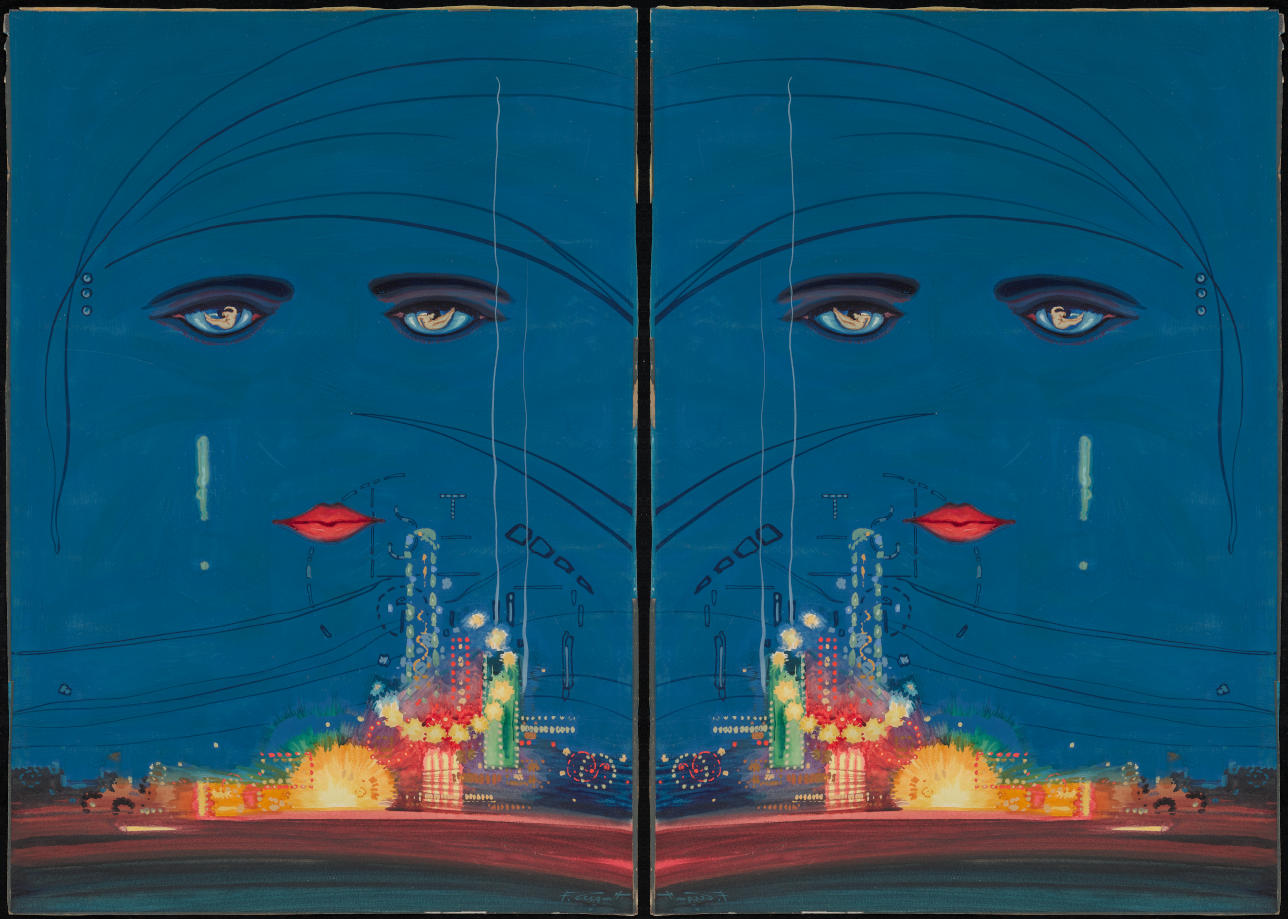
\includegraphics[width=0.27\textwidth]{cover/dustjacket.jpg}
\end{wrapfigure}

Lorem ipsum dolor sit amet, consectetur adipisicing elit, sed do eiusmod
tempor incididunt ut labore et dolore magna aliqua. Ut enim ad minim veniam,
quis nostrud exercitation ullamco laboris nisi ut aliquip ex ea commodo
consequat. Duis aute irure dolor in reprehenderit in voluptate velit esse
cillum dolore eu fugiat nulla pariatur. Excepteur sint occaecat cupidatat non
proident, sunt in culpa qui officia deserunt mollit anim id est laborum. Lorem ipsum dolor sit amet, consectetur adipisicing elit, sed do eiusmod
tempor incididunt ut labore et dolore magna aliqua. Ut enim ad minim veniam,
quis nostrud exercitation ullamco laboris nisi ut aliquip ex ea commodo
consequat. Duis aute irure dolor in reprehenderit in voluptate velit esse
cillum dolore eu fugiat nulla pariatur. Excepteur sint occaecat cupidatat non
proident, sunt in culpa qui officia deserunt mollit anim id est laborum.

% Do not sort citations; this is done manually in ownPublications.bib
\begin{refcontext}[sorting=none]
% mark everything in bibliography lists as cited
\nocite{*}
% print all articles
\printbibliography[heading=subbibliography, title={Peer-reviewed Journal Publications}, type=article]
% print all non-articles
\printbibliography[heading=subbibliography, title={Other Scientific Publications}, nottype=article]
\end{refcontext}	


\end{refsection}

\cleardoublepage
\phantomsection
\chapter{PE\&RC Training and Education Statement}

\begin{wrapfigure}{r}{.35\textwidth}
    \centering
    
\includegraphics[width=4.6cm,height=4.6cm]{PERC_logo.pdf}
\end{wrapfigure}

With the training and education activities listed below the PhD candidate has complied with the requirements set by the C.T. de Wit Graduate School for Production Ecology and Resource Conservation (PE$\&$RC) which comprises of a minimum total of 32 ECTS (= 22 weeks of activities) 

\bigskip

\subsection*{Review/project proposal (9 ECTS)}
\begin{itemize}[nolistsep]
    \item \dots
\end{itemize}

\subsection*{Post-graduate courses (4 ECTS)}
\begin{itemize}[nolistsep]
    \item \dots
    \item \dots
\end{itemize}

\subsection*{Laboratory training and working visits (4.5 ECTS)}
\begin{itemize}[nolistsep]
    \item \dots
    \item \dots
    \item \dots
\end{itemize}

\subsection*{Invited review of journal manuscripts (4 ECTS)}
\begin{itemize}[nolistsep]
    \item \dots
    \item \dots
\end{itemize}

\subsection*{Competence, skills and career-oriented activities (7.92 ECTS)}
\begin{itemize}[nolistsep]
    \item \dots
    \item \dots
    \item \dots
\end{itemize}

\subsection*{PE\&RC Annual meetings, seminars and PE\&RC weekend/retreat (2.1~ECTS)}
\begin{itemize}[nolistsep]
    \item \dots
    \item \dots
\end{itemize}

\subsection*{Discussion groups/local seminars or scientific meetings (10.6 ECTS)}
\begin{itemize}[nolistsep]
    \item \dots
    \item \dots
\end{itemize}

\subsection*{International symposia, workshops and conferences (24~ECTS)}
\begin{itemize}[nolistsep]
    \item \dots
    \item \dots
    \item \dots
\end{itemize}

\subsection*{Lecturing/supervision of practicals/tutorials (21.9~ECTS)}
\begin{itemize}[nolistsep]
    \item \dots
    \item \dots
\end{itemize}

\subsection*{BSc/MSc thesis supervision (24 ECTS)}
\begin{itemize}[nolistsep]
    \item \dots
    \item \dots
    \item \dots
\end{itemize}


\fancyhead{}
\renewcommand{\headrulewidth}{0pt}
\cleartoleftpage

\vspace*{1cm}
The research described in this thesis was financially supported by <name financer>.

Financial support from Wageningen University and <name financier> for printing this
thesis is gratefully acknowledged.


\vspace*{\fill}
Cover design by Name of the designer

Printed by <name printing company> on FSC-certified paper <optional>

\end{document}
